\section{Einleitung}
SAP HANA ist eine Datenbank mit In-Memory-Technik, die von der Firma SAP und dem
Hasso-Plattner-Institut ab dem Jahr 2006 entwickelt wurde und seit 2011 kommerziell
verfügbar ist. Inzwischen ist HANA bei bei mehreren tausend SAP-Kunden im Einsatz.

Die vorliegende Arbeit gibt eine Einführung in einige wesentlichen
Techniken von HANA, und arbeitet die Vorteile der Spaltenorientierung
anhand von experimentellen Messungen heraus.

Im zweiten Abschnitt wird kurz auf die Geschichte und Entwicklung von HANA eingegangen und
einige Kernaspekte der In-Memory-Technologie näher vorgestellt, 
wie die spaltenorientierte Speicherung und Wörterbuch-Kodierung.

Im Abschnitt drei wird anhand von konkreten Benchmarks die Leistung von 
zeilenorientierter und spaltenorientierter Speicherung bei verschiedenen
Einsatzszenarien verglichen.

Im letzten Abschnitt wird ein kritisches Fazit gezogen und ein Ausblick auf weitere 
mögliche Untersuchungen gegeben. Für die Erstellung dieser Arbeit wurde auf 
relevante Fachliteratur zurückgegriffen und im Internet recherchiert. 
Die Benchmark-Messungen wurden auf leistungsfähigen Server-Computern durchgeführt, 
die von SAP im Rahmen der SAP HANA Cloud Platform zur Verfügung gestellt werden.

\section{Motivation und Entwicklung von HANA}
\subsection{Problemstellung}
Seit dem Aufkommen der ersten Datenbank-Systeme in den 70er-Jahres ist eines der
grossen Probleme die geringe Zugriffsgeschwindigkeit der Datenspeicher.
Bei den hierfür eingesetzten Festplatten (HDD) liegt die Latenz für einen Datenzugriff
um viele Grössenordnungen über der Latenz für Zugriffe auf den Arbeitsspeicher (RAM)
des Computers. Im Laufe der Jahrzehnte hat sich diese Diskrepanz immer weiter verschärft.
Seit den 70er-Jahren hat sich die Leistung von CPUs und des RAM millionenfach erhöht,
aber die Zugriffsgeschwindigkeit von Festplatten hat sich nur von 100 ms auf ca. 
10 ms verringert. In diesen 10 ms Wartezeit vergehen bei einer modernen CPU ca. 30 Mio. Takte,
könnte eine Mehrkern-CPU hunderte Millionen Operationen ausführen und 1 GB 
Daten aus dem Arbeitsspeicher lesen.\footnote{vgl. \cite{Intel2016}}

Seit jeher wird in der Datenbank- und Anwendungsentwicklung versucht, dieses 
Missverhältnis durch verschiedene technische Maßnahmen abzumildern, etwa durch 
Caching auf den mehreren Ebenen, durch Anlegen von Indizes mit Baumstruktur oder
auch auf Seite der Anwendungsprogramme, z.B. durch aufwendiges Vorberechnen von diversen Datenaggregaten.
All diese Zusatzmaßnahmen erhöhen die Komplexität der IT-Systeme, den Entwicklungsaufwand,
die Fehleranfälligkeit und binden wertvolle Ressourcen in den verschiedensten Bereichen.

\subsection{Entwicklung moderner Hardware}
In den 2000er-Jahren fanden zunehmend Multi-Core-Prozessoren Verbreitung, also 
CPUs mit mehreren Rechenkernen auf einem Chip. Gleichzeitig wurde Arbeitsspeicher
so günstig, dass Systeme mit mehreren Gigabyte RAM erschwinglich wurden.
So wurde es erstmals theoretisch möglich, eine ganze Unternehmensdatenbank
kommplett im RAM vorzuhalten und auf den Festplattenspeicher als primären
Datenspeicher zu verzichten. Ab 2006 wurde bei der SAP und dem Hasso-Plattner-Institut (HPI) an
dieser Idee gearbeitet, das Potential der verfügbaren Hardware sollte optimal ausgeschöpft
werden ohne durch langsame Festplatten ausgebremst zu werden.\footnote{vgl. \cite{Plattner2015} S.3} Gleichzeitig
würde sich die Komplexität der Systeme deutlich reduzieren und dadurch weitere
Ressourcen frei werden lassen.

Zu diesem Zeitpunkt hatte man bei SAP bereits 
Erfahrung gesammelt mit \textit{TREX}, einer In-Memory-Datenbank mit Column-Store zur Text-Analyse, 
mit \textit{P*Time}, einer einer In-Memory-Datenbank mit Row-Store und mit \textit{MaxDB}, einer
konventionellen relationalen Enterprise-Datenbank auf der auch SAP ECC betrieben werden kann.\footnote{vgl. \cite{Plattner2015} S.5}
Das HPI erhielt Zugang zum Quelltext dieser Datenbank-Systeme und entwickelte einen 
Prototyp der In-Memory-Datenbank für den Unternehmenseinsatz mit dem Namen \textit{SanssouciDB}.
Dieser vielversprechende Prototyp wurde bei SAP zu einem marktfähiges Produkt 
weiterentwickelt, 2010 der Öffentlichkeit vorgestellt und als SAP HANA
ab 2011 kommerziell vertrieben. Anfangs war HANA nur als Appliance erhältlich, 
also eine Kombination von genau aufeinander abgestimmter Software und Hardware.
Inzwischen kann HANA aber auch auf zertifizierten Servern betrieben werden 
(Tailored Data Center Integration). 
Typische HANA-Server haben heute 128 GB bis 12 TB RAM und bis zu 8 Prozessoren mit insgesamt 
einigen Dutzend bis über 100 CPU-Cores.\footnote{vgl. \cite{SAP2016}}

Um die Persistenz der Daten zu gewährleisten kann auch bei einer In-Memory-Datenbank
nicht ganz auf herkömmliche Massenspeicher verzichtet werden. Festplatten oder SSD
sind bei HANA aber nicht mehr der primäre Speicher sondern werden benötigt, 
um regelmäßig Snapshots der Datenbank anzulegen und um alle 
Schreibzugriffe in Log-Dateien abzuspeichern. So kann nach einem Stromausfall der Zustand
der Datenbank aus dem letzten Snapshot und allen Logs seit diesem Zeitpunkt 
zuverlässig  wieder hergestellt werden.

Mit dem Wegfall des relativ langsamen Massenspeichers ist nun der Arbeitsspeicher
der neue Flaschenhals für den Datentransport. Im Vergleich zu den 10 ms einer Festplatte ist der Zugriff
auf DRAM mit ca. 100 ns zwar um viele Grössenordnungen schneller, jedoch beträgt die 
Zykluszeit aktueller Prozessoren nur etwa 0,3 ns. Bei einem Zugriff auf den DRAM-Arbeitspeicher
muss die CPU also immer noch mehrere hundert Takte auf das Ergebnis warten. Aus diesem Grund
sind zwischen CPU und DRAM-Arbeitsspeicher mehrere Stufen von kleinen aber schnellen
Cache-Speichern aus SRAM geschaltet. Von dem schnellsten Level-1-Cache (L1) kann bei einem
Treffer (Cache-Hit), also wenn sich die Daten der angefragten RAM-Adresse im Cache befinden, 
mit 0,5 ns Latenz gelesen werden. Auf den grösseren Level-2-Cache kann noch mit 7 ns
Verzögerung zugegriffen werden. \footnote{vgl. \cite{Plattner2015hpi} S.29} Meist kommt auch
noch ein L3-Cache  zum Einsatz, sodass pro CPU bis zu 60 MB Cache zur Verfügung stehen.\footnote{vgl. \cite{Intel2016}}
Bei einem Cache-Miss, also wenn sich die angeforderten Daten noch nicht im Cache befinden,
muss die CPU aber mindsten 100 ns auf den DRAM warten, ein Cache-Miss sollte also möglichst vermieden werden.

Der Cache wird in Blöcken zu je 64 Byte, den sogenannten Cache-Lines, verwaltet. 
Diese Cache-Lines werden immer zusammen am Stück aus dem Arbeitsspeicher in den Cache geladen,
zwar mit der entsprechenden Latenz, aber einer hohen Bandbreite.
Daten innerhalb dieser Cache-Line können also von der CPU sehr schnell gelesen werden.
In der Zwischenzeit kann aus dem Arbeitsspeicher schon die nächste Cache-Line geladen werden
(Prefetching). Zusammenhängende Speicherbereiche können so mit einer Geschwindigkeit 
von 4 MB / ms von einem Core gelesen und gescannt werden. Bei einer 15-Kern-CPU ist 
das eine Scangeschwindigkeit 60 GB pro Sekunde, also bei einem 8-Sockel-System 480 GB pro Sekunde.\footnote{vgl. \cite{Plattner2015hpi} S.29}

\subsection{Spaltenorientierung}

Eine Tabelle in einer Datenbank ist eine theoretische, 2-dimensionale Struktur,
die auf den linear addressierten Speicher eines Computers abgebildet werden muss. Diese
Abbildung kann sinnvoll auf zwei Arten geschehen: zeilenorientiert und spaltenorientiert.
Bei der zeilenorientierten Speicherung werden alle Attribute eines Datentupels hintereinander abgelegt, z.B.
\texttt{[Max,Huber,m,81234,München,Müllerstraße,12]} und daran anschliessend das nächste Tupel.
Diese Art der Speicherung orientiert sich im Prinzip noch an der Datenverarbeitung mit Lochkarten oder Magnetbändern,
wo ein schneller wahlfreier Zugriff wie bei Festplatten nicht möglich war.

Bei der spaltenorientierten Speicherung hingegen wird ein Attribut aller Tupel zusammen in einem Attribut-Vektor abgelegt, z.B.
\texttt{[Annett,Max,Stefan,Susanne]} und daran anschliessend die anderen Attributvektoren.
Die hohe Leseleistung von zusammenhängenden Speicherbereichen, bzw. die schlechte
Leistung bei verteilten Zugriffen sind der Grund, warum analytische Datenbank-Abfragen bei 
spaltenorientierter Speicherung (Column-Store) deutlich schneller sind als bei zeilenorientierter Speicherung
(Row-Store). Bei dieser Art von Abfragen müssen üblicherweise große Mengen eines
oder mehrer Attribute verarbeitet werden, z.B. mit Filter- oder Aggregationsfunktionen.
Demgegenüber ist die zeilenorienterte Speicherung (Row-Store) im Vorteil, wenn viele oder alle Attribute 
(Spalten) eines oder mehrere Datensätze gelesen oder geschrieben werden (Row Operation).
Abbildung \ref{rscs} veranschaulicht die Speicherzugriffsmuster dieser beiden Betriebsmodi
bei Row- und Column-Store.

\begin{figure}[h]
\centering
\includegraphics[width=.9\textwidth]{img/rs-cs2.png}
\caption[Zugriffsmuster bei Row-Store und Column-Store]{Zugriffsmuster bei Row-Store und Column-Store\footnotemark}
\label{rscs}
\end{figure}
\footnotetext{Quelle: eigene Darstellung nach \cite{Plattner2015hpi} S.62}


\subsection{Wörterbuch-Kodierung und Datenkompression}
Bei einer In-Memory-Datenbank wie SAP HANA ist wie bereits beschrieben nicht mehr die Festplatte (HDD oder SSD) der
Flaschenhals sondern der Arbeitsspeicher (RAM). Aus dem Arbeitsspeicher können die 
Daten jedoch nicht so schnell geladen werden, wie der Prozessor (CPU) sie bearbeiten kann.
Bei den heute üblichen Multicore-Prozessoren, mit vielen Rechenkernen pro Prozessor-Chip 
verstärkt sich dieser Effenkt noch einmal deutlich.

Die Datenbank arbeitet also um so langsamer, je mehr Daten vom Hauptspeicher 
gelesen (bzw. dorthin wieder geschrieben) werden müssen.
Am schnellsten kann die CPU arbeiten, wenn die Daten aus dem internen Cache gelesen
werden können, der jedoch in der Grösse beschränkt ist.
Daher wird mit verschiedenen Techniken versucht, die Datenmenge zu reduzieren.
Eine dieser Techniken ist die Wörterbuch-Kodierung (engl. dictionary encoding).
Dabei wird in den Tabellenspalten nicht der Datenwert selbst gespeichert, sondern eine
Integer-Zahl, die diesen Wert eindeutig repräsentiert. Zusätzlich gibt es für jede Spalte 
ein eigenes Wörterbuch (dictionary), mit dem die Integer-Werte wieder dem 
eigentlichen Datenwert zugeordnet werden können. 
Sollen z.B. Personendaten wie 
Name und Adresse in einer Tabelle abgelegt werden, kommen viele Werte mehrfach vor, 
es gibt also Redundanzen im Datenbestand.
Am Beispiel einer Spalte mit Vornamen wird in Abbildung \ref{dictenc} das Prinzip der Kodierung mit einem Wörterbuch verdeutlicht.

\begin{figure}[h]
\centering
\includegraphics[width=.9\textwidth]{img/dict-enc.png}
\caption[Prinzip der Wörterbuch-Kodierung]{Prinzip der Wörterbuch-Kodierung\footnotemark}
\label{dictenc}
\end{figure}
\footnotetext{Quelle: eigene Darstellung nach \cite{Plattner2015hpi} S.39}

So gibt es z.B. in Deutschland 11116 unterschiedliche Gemeinden. 
\footnote{vgl. \cite{Statista2014}}
Mit einer Wörterbuch-Kodierung kann jede Gemeinde mit einer 14-Bit-Zahl 
dargestellt werden, denn 2\textsuperscript{14} = 16384.
Wenn die Ortsnamen als normaler Text abgespeichert würden, so müssten dafür 32 Byte
vorgesehen werden (längster Ortsname in Deutschland). Bei einer Kundendatei von
20 Mio. Personen wäre das Datenvolumen der Spalte Ort 20 Mio. * 32 Byte = 640 MB.

Mit Wörterbuch-Kodierung hingegen werden nur 20 Mio. * 14 Bit = 280 MBit = 35 MB benötigt. 
Hinzu kommt noch das Wörterbuch mit maximal 11116 * 32 Byte = 355712 Byte = 0,35 MB.
Der Komprimierungsfaktor in diesem Beispiel wäre also 640MB/35,35MB = 18,1.

Allgemein kann für geschäftliche Daten wie in einem SAP-System von einem
Komprimierungsfaktor von etwa 1:5 ausgegangen werden. Duch den Wegfall von Indizes und 
vorberechneten Daten-Aggregaten werden etwa weitere 50\% Datenvolumen eingespart.
Ingesamt ist das Datenvolumen also nur ca. 1/10 einer konventionellen relationalen 
Datenbank wie Oracle, MaxDB oder MS-SQL-Server.
\footnote{vgl. \cite{Plattner2015} S.22}

Mit klassischen Methoden zur Datenkompression kann das benötigte Datenvolumen 
der kodierten Spalten noch weiter reduziert und somit die Geschwindikeit erhöht werden.
Bei HANA kommen dazu leichtgewichtige Algorithmen zum Einsatz wie die Lauflängenkodierung (run-length encoding).
\footnote{vgl. \cite{Plattner2015hpi} S.47}
Komplexe Algorithmen wie zip lohnen sich nicht, da der Aufwand zur Dekomprimierung
grösser ist als die erzielte Bandbreiteneinsparung.
Für manche Kompressionsmethoden muss eine Spalte sortiert sein, wobei eine Tabelle
natürlich immer nur nach einer Spalte sortiert sein kann.
Der zusätzliche Vorteil einer sortierten Spalte ist, daß der Zugriff auf ein bestimmtes 
Element daraus mittels binärer Suche in logarithmischer Zeit (Komplexität O(log n)) 
erfolgen kann. Es ist also weder ein zusätzlicher Index von ein voller Tablescan erforderlich.

\subsection{Parallelverarbeitung}

Moderne Prozessoren enthalten normalerweise mehrere Rechenkerne 
(z.B. aktuelle Intel Xeon bis zu 24 physische Kerne)\footnote{vgl. \cite{Intel2016}}
und Server-Computer können mehrere Prozessoren besitzen\footnote{vgl. \cite{Intel2014}}.
Server mit 80 Rechernkernen und mehr sind daher heute nicht unüblich\footnote{vgl. \cite{Plattner2015hpi}}.
SAP HANA kann das Potential dieser Rechenleistung voll ausschöpfen, da es von
Beginn an mit Fokus auf Parallelverarbeitung entwickelt wurde.
Wenn z.B. bei einer SQL-Abfrage mehrere Spalten ausgewertet werden müssen, 
so kann jeweils ein Kern eine Spalte bearbeiten. Aber auch wenn nur eine Spalte bearbeitet wird
können mehrere Kerne gleichzeitig daran arbeiten und z.B. die Summe berechnen.
Die Einzelergebnisse werden danach zum Endergebnis zusammengeführt
(Abbildung \ref{paral}).
\begin{figure}[h]
\centering
\includegraphics[width=.7\textwidth]{img/parallelverarbeitung.png}
\caption[Parallelverarbeitung im Column-Store]{Parallelverarbeitung im Column-Store\footnotemark}
\label{paral}
\end{figure}
\footnotetext{Quelle: Prassol, P. (2015)}
Sehr grosse Tabellen im Terrabyte-Bereich können sogar über mehrere Server
(sog. Nodes) verteilt werden (Scale-out). Diese sind mit einem Hochgeschwindigkeits-Netzwerk
verbunden und tauschen untereinander Abfragen, Daten und Ergebnisse aus.
Die Aufteilung kann spaltenweise oder zeilenweise (Partitionierung) erfolgen.
Auch eine gemischte Aufteilung ist möglich: z.B. Spalten U, V und W sind klein genug
und passen auf Server 1, Spalte X ist gross und liegt auf Server 2 und Spalte Y 
ist so gross, dass sie via Partitionierung auf Server 3 bis 10 verteilt wird.
So können ohne Weiteres 1000 Rechenkerne eine Abfrage gleichzeitig bearbeiten
die Verarbeitungsleistung steigt nahezu linear.\footnote{vgl. \cite{SAP2014}}

\section{Experimenteller Leistungs-Vergleich von zeilen- und spaltenorientierter Speicherung}
\subsection{Testaufbau}
Für den Geschwindigkeisvergleich von Row-Store und Column-Store wurde die frei
zugängliche Entwicklungs- und Testumgebung der SAP HANA Cloud Platform (HCP) eingesetzt.\footnote{\url{https://hcp.sap.com}}
Hier kann eine bis zu 1 GB grosse HANA-Datenbank auf leistungsfähigen Server-Computern 
der SAP betrieben werden. 
Für die Tests wurden mit einem Ruby-Script
\footnote{\url{https://www.kurmis.com/csv-faker}}
genau 5 Mio. Personendatensätze mit Zufallsdaten generiert
und in einer CSV-Datei abgespeichert. Die Datensätze bestehen aus Name, Anschrift,
Email, Größe(cm), Gewicht(kg) und Geburtsdatum, wobei Größe und Gewicht jeweils normal-verteilt
sind und miteinander korrelieren:

\begin{scriptsize}
\begin{verbatim}
1;Fatma;Maier;Violastr.;1;19760;Mainburg;fatma_maier@greenfelderdamore.us;155;57;1974-06-17
2;Marc;Elsner;Ferdinandstr.;53;57315;Alzey;marc_elsner@anderson.biz;183;88;1931-02-10
3;Noelle;Hahn;Beckstr.;6;57109;Freilassing;hahn_noelle@kreiger.co.uk;168;44;1982-01-28
4;Mona;Wagner;Connerstr.;14;48256;Leichlingen;mona.wagner@emardpadberg.name;171;73;1942-09-13
\end{verbatim}
\end{scriptsize}

Für den Zugriff auf die Datenbank kam die Entwicklungsumgebung \textit{Eclipse} in Verbindung 
mit den \textit{SAP HANA Cloud Platform Tools} zum Einsatz.
\footnote{\url{https://tools.hana.ondemand.com}}

In der Datenbank wurden 2 Tabellen für die Personendaten angelegt, eine Tabelle 
mit Row-Store (RPERSON) und eine Tabelle mit Column-Store (CPERSON): 

\begin{verbatim}
CREATE COLUMN TABLE "CPERSON" (
    "ID" INTEGER CS_INT NOT NULL ,
    "FIRST_NAME" NVARCHAR(20) NOT NULL ,
    "LAST_NAME" NVARCHAR(20) NOT NULL ,
    "STREET" NVARCHAR(20) NOT NULL ,
    "STR_NUM" SMALLINT CS_INT NOT NULL ,
    "ZIP" VARCHAR(5) NOT NULL ,
    "CITY" NVARCHAR(30) NOT NULL ,
    "EMAIL" NVARCHAR(60) NOT NULL ,
    "HEIGHT" TINYINT CS_INT NOT NULL ,
    "WEIGHT" TINYINT CS_INT NOT NULL ,
    "BIRTHDAY" DAYDATE CS_DAYDATE NOT NULL ,
    PRIMARY KEY ("ID")) UNLOAD PRIORITY 5 AUTO MERGE 
;
\end{verbatim}

Die Tabelle mit Row-Store wurde analog mit \texttt{CREATE ROW TABLE} angelegt 
(\texttt{CS\_INT} und \texttt{CS\_DAYDATE} können auch weggelassen werden, diese Datentypen werden von HANA
beim Erstellen der Tabellen automatisch verwendet).
Als Tabellenbezeichner wird im Folgenden nur \texttt{PERS} verwendet, und soll als 
Platzhalter für CPERSON und RPERSON verstanden werden.\\
Die CSV-Datei mit den 5 Mio. Test-Datensätze wurde mit Hilfe von \textit{Eclipse} und 
den \textit{SAP HANA Cloud Platform Tools} in eine der beiden Tabellen übertragen 
(Abbildung \ref{import})
und anschließend von dort mittels SQL in die zweite Tabelle kopiert, so dass beide
Tabellen exakt die gleichen Daten enthalten.

\begin{figure}[h]
\centering
\includegraphics[width=.99\textwidth]{img/import.png}
\caption[Import von CSV-Daten mit Eclipse]{Import von CSV-Daten mit Eclipse\footnotemark}
\label{import}
\end{figure}
\footnotetext{Quelle: eigener Screenshot}

Die eigentlichen Datenbank-Abfragen für den Benchmark wurden aus Eclipse heraus 
auf jeder Tabelle jeweils 4 mal ausgeführt und von deren Ausführungszeiten auf dem 
Server (server processing time) t1-t4 der Mittelwert Øt bestimmt.\footnote{siehe Anhang 1: Benchmark-Daten}
Die gemessenen Werte lagen durchweg im Millisekunden-Bereich und waren mit geringen
Schwankungen reproduzierbar. Es wurden verschiedene SQL-Abfragen vom analytischen Typ (OLAP) 
und vom transaktionalen Typ (OLTP) gestellt und gemessen, jedoch keine Schreibzugriffe wie
INSERT oder UPDATE.
Anschließend wurde jeweils noch ein Index zu den Spalten \texttt{HEIGHT} und 
\texttt{WEIGHT} angelegt (Abfragen Q und R) und ausgewählte OLAP- und OLTP-Abfragen
noch einmal zum Vergleich ausgeführt.

\subsection{OLAP - analytische Abfragen}
Die analytischen Datenbank-Abfragen verwenden typischerweise Aggregationsfunktionen
wie COUNT(), SUM(), AVG(), MIN(), MAX() und arbeiten nur auf wenigen ausgewählten 
Spalten, die Ergebnismenge ist in der Regel klein.\\
Mit Fokus auf diese Art von Abfragen wurde der Column-Store von SAP HANA entwickelt.
Diese Abfragen auf die Column-Store-Tabelle werden dementsprechend auch schneller 
von dem DBMS bearbeitet als Abfragen auf die Row-Store-Tabelle.

\subsection{OLTP - Transaktionale Abfragen}
Transaktionale Abfragen lesen in der Regel viele Spalten oder alle Spalten einer
Tabelle (SELECT *) und haben einen einzelnen Datensatz oder mehrere Zeilen als
Ergebnismenge. Diese Art von Abfragen werden im laufenden Geschäftsbetrieb verwendet
um z.B. Detaildaten zu einem Kunden oder eine Liste von Kunden anzuzeigen.
Hier ist der Row-Store vorteilhaft, da die einzelnen Attribute eines Datensatzes
im Speicher nah beieinander liegen und daher schnell darauf zugegriffen werden kann.

Die Selektion eines einzelnen Datensatzen erfolgt bei beiden Tabellen so schnell (<1ms),
dass ein sinnvoller Vergleich nicht möglich ist. Deswegen wurden die Abfragen so 
gewählt, dass sie als Ergebnismenge 1000 Tupel zurückliefern, wie z.B. 
\texttt{select * from PERS where id <= 1000} (Abfragen O,P,U,V).
Bei den verwendeten Abfragen erfolgt die Selektion über den Primärschlüssel \texttt{ID}
und ist daher sehr schnell (Nutzung eines Index).

\subsection{Diskussion}
Die analytischen OLAP-Abfragen werden von dem Column-Store etwa eine Grössenordnung
schneller bearbeitet als von dem Row-Store. Der Beschleunigungsfaktor variiert aber 
stark zwischen den einzelnen Abfragen und reicht von 1,4 (Abfrage E: 
\texttt{select sum(weight) from PERS}) bis zu Faktor 170 (Abfrage M: \texttt{select count(*) from PERS where
height = 210 and weight=110}). Hier zeigt sich, dass die Spalten in einem
Column-Store viel schneller gescannt werden können.\\
Bei Abfrage N (\texttt{select * from PERS where height=210 and weight=110}) werden
über 300 Tupel mit allen Spalten als Ergebnis zurückgeliefert und trotzdem ist hier
der Column-Store noch um Faktor 16 schneller als der Row-Store. Das liegt daran,
dass hier die Selektion nicht über den Primärschlüssel erfolgt, sondern die Spalten
\texttt{height} und \texttt{weight} gescannt werden müssen, was beim Column-Store
deutlich schneller erfolgen kann.\\
Bemerkenswert ist die nur geringe Beschleunigung um Faktor 1,4 bei der Summenfunktion
\texttt{SUM()} bei Abfrage E. Bei Einsatz eines Column-Store ist die Funktion 
erstaunlicherweise nur halb so schnell wie
\texttt{MIN()}, \texttt{MAX()} oder \texttt{AVG()}, im Row-Store jedoch ist die 
Summen-Funktion etwa um eine Größenordnung schneller als die  anderen Aggregatsfunktionen.
Diese Besonderheit sollte noch genauer untersucht werden, da SUM() eine wichtige 
SQL-Funktion ist die in realen Geschäftsanwendungen oft verwendet wird.

\begin{figure}[h]
\centering
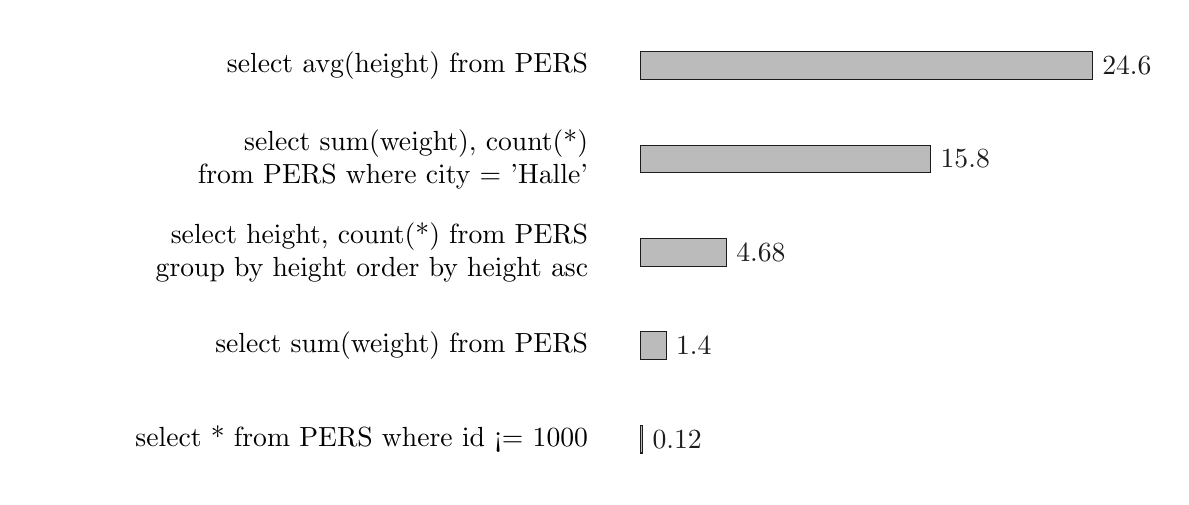
\begin{tikzpicture}
  \selectcolormodel{gray}
  \begin{axis}[
    xbar,
    y axis line style = { opacity = 0 },
    axis x line       = none,
    tickwidth         = 0pt,
    yticklabel style={text width=7cm,align=right},
%    enlarge y limits  = 0.2,
%    enlarge x limits  = 0.02,
    symbolic y coords = {
        {select * from PERS where id <= 1000},
        {select sum(weight) from PERS}, 
        {select height, count(*) from PERS group by height order by height asc},
        {select sum(weight), count(*) from PERS where city = 'Halle'}, 
        {select avg(height) from PERS}
        },
    nodes near coords,
  ]
  \addplot coordinates { 
    (24.6,{select avg(height) from PERS})
    (15.8,{select sum(weight), count(*) from PERS where city = 'Halle'}) 
    (4.68,{select height, count(*) from PERS group by height order by height asc}) 
	 (1.40,{select sum(weight) from PERS}) 
     (0.12,{select * from PERS where id <= 1000})};
  \end{axis}
\end{tikzpicture}
\caption[Performance Column-Store / Row-Store]{Performance Column-Store / Row-Store\footnotemark}
\label{bench}
\end{figure}
\footnotetext{Quelle: eigene Darstellung}

Abbildung \ref{bench} zeigt exemplarisch die relative Performance von Column-Store und Row-Store für einige SQL-Abfragen.
Beispielsweise ist \texttt{select avg(height) from PERS} mit dem Column-Store 24,6 mal schneller als mit dem Row-Store.

Das Anlegen der Indizes auf der CS-Tabelle erfolgt sehr schnell (ca. 150ms), 
allerdings profitiert der Column-Store davon kaum, die Ausführungszeiten verbessern
sich nicht signifikant. (s. Tabelle \ref{tab:indizes})

\begin{table}[!ht]
  \centering
\begin{verbatim}
Req#          SQL                     Colum-Store       Row-Store
                                     ohne/mit Index    ohne/mit Index
_____________________________________________________________________
N,S:  select * from PERS where 
         height=210 and weight=110    3,75/ 2,18 ms   61,78/  0,61 ms
_____________________________________________________________________
A,T:  select MIN(height) from PERS   11,56/10,62 ms  185,81/185,56 ms
\end{verbatim}
  \caption{Einfluss von Indizes auf die Performance bei Row-Store und Column-Store}
  \label{tab:indizes}
\end{table}

Bei der Abfrage T mit der Funktion MIN() findet der Index offenbar keine 
Verwendung im Ausführungsplan, die Ausführungzeiten haben sich durch den
Index im Column-Store und im Row-Store nicht verändert.\\
Bei der RS-Tabelle dauert die Erstellung der Indizes deutlich länger (>6s), 
jedoch kann der Row-Store teilweise deutlich von den Indizes profitieren.
Bei Abfrage S, welche 323 vollständige Tupel selektiert, kann 
die Ergebnismenge 100 mal schneller bestimmt und geliefert werden: in 0,61ms statt 61,8ms.
Bei einem realen Anwendungsfall kommen solche Indizes normalerweise auch zur
Anwendung, wenn über die entsprechenden Spalten häufig selektiert wird. 
Deswegen müssen für einen realistischen Geschwindigkeitsvergleich auch 
Indizes berücksichtigt werden.\\
Hier wird also deutlich, dass auch der Row-Store seine Vorteile hat, und zwar
immer dann, wenn die Ergebnismenge viele Spalten oder sogar die kompletten
Tupel enthält. Durch die Lokalität der Daten eines Tupels kann das ganze Tupel
sehr schnell aus dem Speicher gelesen werden. 
Der Column-Store fällt hier zurück, weil die Attribute eines Tupels an relativ 
weit entfernten Speicherstellen abgelegt sind und erst wieder zu einem Datensatz
zusammengefügt werden müssen (Tuple Reconstruction).
Je mehr Zeilen die Ergebnismenge hat, umso deutlicher ist der Row-Store im Vorteil.

Dieser kleine Geschwindigkeitsnachteil des Column-Store im OLTP-Bereich hat in
der Praxis aber kaum Auswirkungen, da hier immer auch noch andere Latenzen in 
den nachgelagerten Systemen auftreten und die transaktionalen Abfragen insgesamt
ja sehr kurz sind. Bei einem Mischbetrieb von OLAP und OLTP sollte also vorzugsweise
mit einem Column-Store gearbeitet werden, denn die Geschwindigkeitsvorteile bei
OLAP-Abfragen überwiegen deutlich.

\section{Fazit und Ausblick}
In der Arbeit wurde ein kurzer Überblick über die In-Memory-Datenbank SAP HANA gegeben.
Es wurde gezeigt, wie und mit welcher Motivation diese neue Technologie bei der 
Firma SAP und dem Hasso-Plattner-Institut entwickelt wurde.
Die beiden Schlüssel-Techniken Spaltenorientierung und Wörterbuch-Kodierung wurden kurz skizziert.
Anhand von synthetischen Benchmarks wurden Row-Store und Column-Store gegenübergestellt
und die jeweiligen Vor- und Nachteile herausgearbeitet. Dabei hat sich die Überlegenheit der
spaltenorientierten Speicherung für analytische Datenbank-Abfragen klar gezeigt.

Die hier ermittelten Ergebnisse sind jedoch nur ein erster Anhaltspunkt.
Für weitergehende systematische Untersuchungen von Row- und Column-Store sollten 
auch die Leistung von Schreibzugriffen gemessen werden sowie die Leistung bei Mischbetrieb 
von Lese- und Schreibzugriffen, wie er ja auch in der Praxis vorkommt.\\
Die in dieser Arbeit verwendete Datenmenge war mit 5 Mio. Datansätzen und 481MB Rohdaten recht klein.
Die gemessenen Zeiten waren daher auch nur sehr kurz. Um aussagekräftigere Messwerte
zu bekommen sollte die Datenmenge noch deutlich grösser sein.
Interessant wäre auch ein Vergleich von SAP HANA mit anderen RDBM auf der gleichen Hardware,
wie Oracle DB, MS SQL-Server, MaxDB, MySQL, Maria-DB oder PostgreSQL welche teilweise auch mit
einem Column-Store betrieben werden können, zum Teil werben deren Anbieter auch mit In-Memory-Technik.
Idealerweise sollte Datenbank-Leistung mit einem standardisierten Test,
wie z.B. TPC gemessen werden, um vergleichbar zu sein.
Der Aufwand dafür sollte aber nicht unterschätzt werden.
